\chapter{Lecture 16: Geometry of Fractional Linear Transformations}

\section{Lines \& Circles}

\begin{example}
    $T(z) = \frac{1}z$\\
    If $f(z) = |z-z_0|^2 - r^2 = 0$, then we can compute $f(T(z)$):
    \begin{align*}
        |z|^2 z\overline{z} - z\overline{z_0} - z_0\overline{z} + |z_0|^2 & = r^2                                                                            \\
        |z|^2 - 2\Re(z\overline{z_0}) + |z_0|^2                           & = r^2                                                                            \\\
        1 - 2\Re(z\overline{z_0}\frac{z}{|z|^2})                          & = \frac{r^2 - |z_0|^2}{|z|^2}                                                    \\
        \text{Then }                                                      & w = \frac{1}z \text{ satisfies}                                                  \\
        |w|^2(r^2 - |z_0|^2)                                              & = 1 - 2\Re(\frac{|w|^2}{w}\overline{z_0}) = 1 - 2\Re(\overline{w}\overline{z_0}) \\
        \rightarrow \Re(\overline{w}\overline{z_0})                       & = \Re(\overline{z_0}w)\end{align*}
    Which is just another circle, unless $z_0 = r$.
    \begin{align*}
        \text{If } r & = |z_0|, \text{ then}      \\
        \Re(wz_0)    & = \frac{1}2 \text{ A line}
    \end{align*}
    Therefore we see that $T(z) = \frac{1}z$ maps circles to lines if and only if $z = 0$ lies on the circle since $T(T(z)) = z$, we also see that $T$ takes lines to circles.
\end{example}

\begin{proposition}
    [Möbius Transformation (Lines \& Circles)]
    Given a circle: $f(z) = |z-z_0|^2 - r^2 = 0$, then $T(z) = \frac{1}{z - a}$ maps the circle to a line if and only if the edge of the circle passes through $a$ so that $|a - z_0| = r$. \\
    The equation of the line is $\Re(wz_0) = \frac{1}2$ where $w = \frac{1}{z - a}$.
\end{proposition}

\begin{figure}[H]
    \centering
    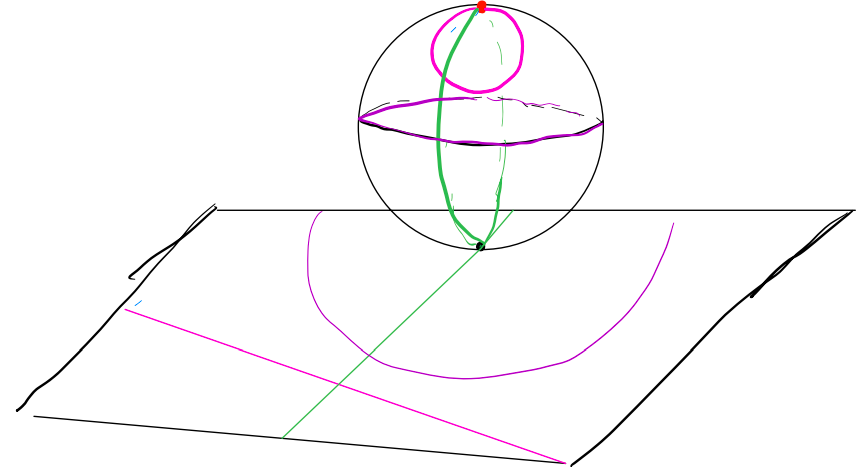
\includegraphics[width=0.5\textwidth]{LECTURE_16/circle-through-infty.png}
    \caption{Circle through $\infty$}
\end{figure}

\begin{lemma}
    If $T$ is a fractional linear transformation, then either $T$ is \underline{linear} or, these exist $T_1, T_3$ are \underline{linear} (i.e. $T_1(z) = a_1z + b_1, T_3(z) = a_3z + b_3$) such that if we take $T_2(z) = \frac{1}{z}$, then:
    \begin{align*}
        T = T_3 \circ T_2 \circ T_1
    \end{align*}
\end{lemma}

\begin{proof}
    $T= \frac{az + b}{cz + d}$, $T$ is linear if and only if $c = 0$, so we assume $c \neq 0$.\\
    \begin{align*}
        T & = \frac{1}{c} \left(\frac{bc - ad}{cz + d} + a\right)
    \end{align*}
    Then we define:
    \begin{align*}
        T_3(z) & = \frac{1}{c} (bc - ad)z + a \\
        T_1(z) & = cz + d
    \end{align*}
\end{proof}

\begin{corollary}
    A fractional linear transformation takes:
    \begin{align*}
        \left\{
        \begin{aligned}
             & \text{Circles or} \\
             & \text{Lines}
        \end{aligned}
        \right\}
         & \xrightarrow{T}
        \left\{
        \begin{aligned}
             & \text{Circles or} \\
             & \text{Lines}
        \end{aligned}
        \right\}
    \end{align*}
\end{corollary}

\begin{proof}
    If $T$ is linear, then $T$ takes lines to lines and circles to circles. If $T$ is not linear, then $T = T_3 \circ T_2 \circ T_1$ where $T_1, T_3$ are linear and $T_2(z) = \frac{1}{z}$ takes lines to circles/lines and circles to lines/circles.
\end{proof}

\section{Conformal Mapping}

\begin{proposition}
    Suppose $z_1(t)$ and $z_2(t)$ are curves in $\mathbb{C}$, (say for $t \in [-1, 1]$) and $z_1(0) = z_2(0) = z_0$. The tangent vector of the curves $z_j(t) = x_j(t) + iy_j(t), \quad j = 1, 2$ is given by:
    \begin{align*}
        z'_j(t) = x'_j(t) + iy'_j(t)
    \end{align*}
    The angle between $z_1, z_2$ at $(t = 0, z_0)$ is given by:
    \begin{align*}
        \theta =  \arg(z'_2(0))- \arg(z'_1(0))
    \end{align*}

    \begin{figure}[H]
        \centering
        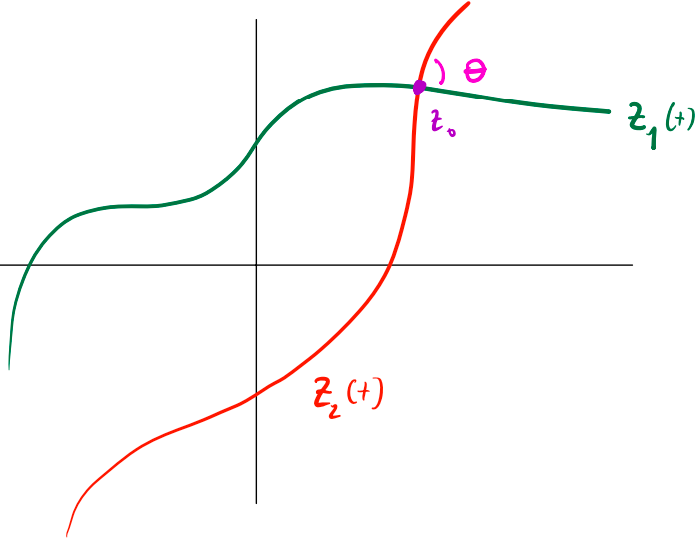
\includegraphics[width=0.5\textwidth]{LECTURE_16/graph.png}
        \caption{Angle between curves}
    \end{figure}

    Now suppose $f$ is an analytic function defined in $|z - z_0| < r$ such that $f'(z_0) \neq 0$. Then:
    \begin{align*}
        w_1(t) & = f(z_1(t)), \quad w_2(t) = f(z_2(t)) \text{ are curves in } \mathbb{C} \\
    \end{align*}

    \begin{figure}[H]
        \centering
        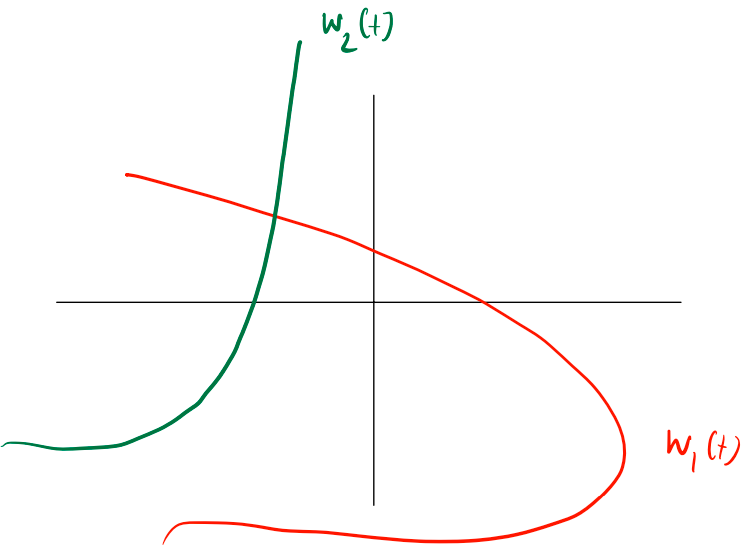
\includegraphics[width=0.5\textwidth]{LECTURE_16/graph2.png}
        \caption{Curves under $f$}
    \end{figure}

    The tangent vector to $w_j(t)$ at $t = 0$ is given by:
    \begin{align*}
        w'_j(0) = f'(z_0)z'_j(0)
    \end{align*}
    And the \underline{angle} between some $w_i, w_j$ is:
    \begin{align}
        \arg(w'_j(0)) = \arg(f'(z_0)) + \arg(z'_j(0)) \quad j = 1, 2
    \end{align}
    so
    \begin{align}
        \arg(w'_2(0)) - \arg(w'_1(0)) = \arg(z'_2(0)) - \arg(z'_1(0))
    \end{align}
    (This is because if $u = u_1\cdot u_2, \quad \arg(u) = \arg(u_1) + \arg(u_2)$)
    also
    \begin{align}
        |w'_j(0)| = |f'(z_0)||z'_j(0)| \quad j = 1,2
    \end{align}
\end{proposition}

\begin{definition}
    [Conformal Map]
    A conformal map $\phi : \mathbb{C} \to \mathbb{C}$ is a map such that
    \begin{enumerate}
        \item if $\gamma_1(t), \gamma_2(t)$ are two curves such that $\gamma_1(0) = \gamma_2(0)$ then
        \item[] Angle between $\gamma_1'(0)$ and $\gamma_2'(0)$ = Angle between $\phi(\gamma_1)'(0)$ and $\phi(\gamma_2)'(0)$
        \item[]
        \item The lengths of tangent vectors are \underline{scaled} by a positive constant
        \item[] $|\gamma_j'(0)|c = |\phi(\gamma_j)'(0)|$
    \end{enumerate}
    Essentially, a conformal map preserves angles, but not necessarily lengths.
\end{definition}

\begin{theorem}
    If $f$ is analytic near $z_0$, and $f'(z_0) \neq 0$, then $f$ is a conformal map near $z_0$.
\end{theorem}

\begin{example}
    [Map Projections]
    The mercator projection is conformal, so it preserves \underline{compass angles} and hence very useful for navigation.
\end{example}